\chapter{Dữ liệu tin tức}
\label{ch:M5L2LessonNotes}

\section*{Lesson Notes}

MODULE 5 \textbar{} BÀI 2

{\small
\begin{longtable}[]{@{}
  >{\raggedright\arraybackslash}p{(\columnwidth - 2\tabcolsep) * \real{0.5000}}
  >{\raggedright\arraybackslash}p{(\columnwidth - 2\tabcolsep) * \real{0.5000}}@{}}
\toprule\noalign{}
\endhead
\bottomrule\noalign{}
\endlastfoot
\textbf{Thời gian đọc} & 45 phút \\
\textbf{Kiến thức nền tảng} & Quen thuộc với lập trình Python: cú pháp Python cơ bản, xử lý dữ liệu, DataFrame, yfinance, sklearn; Các khái niệm tài chính cơ bản: cổ phiếu, cảm xúc thị trường, quản trị rủi ro, chiến lược giao dịch, phân tích cảm xúc \\
\textbf{Từ khóa} & Phân rã ma trận không âm (NMF), trích xuất đặc trưng, biểu diễn theo bộ phận (parts-based representation), phân tích cảm xúc, xử lý ngôn ngữ tự nhiên (NLP), phân tích cảm xúc, mô hình hóa chủ đề, FinBERT, NMF, TF-IDF \\
\end{longtable}
}

\begin{center}\rule{0.5\linewidth}{0.5pt}\end{center}

\emph{Trong bài học này, chúng ta trình bày cách sử dụng dữ liệu tin tức và các kỹ thuật xử lý ngôn ngữ tự nhiên (NLP) cho phân tích tài chính, cụ thể là đối với Microsoft. Chúng ta sẽ khám phá các nguồn tin tức khác nhau, thực hiện phân tích cảm xúc bằng FinBERT, và sử dụng mô hình hóa chủ đề (NMF) để khám phá các chủ đề ẩn trong tin tức. Mục tiêu là thu được những hiểu biết có thể giúp đưa ra các quyết định tài chính sáng suốt hơn.}

\begin{lstlisting}[language=Python,escapeinside={(*@}{@*)}]
import torch
\end{lstlisting}

\begin{lstlisting}[language=Python,escapeinside={(*@}{@*)}]
# Loading libraries

import datetime
import feedparser
import matplotlib.pyplot as plt
import numpy as np
import pandas as pd
import requests
import yfinance as yf

from datetime import datetime, timedelta
from scipy.special import softmax
from sklearn.feature_extraction.text import TfidfVectorizer
from sklearn.decomposition import NMF
from sklearn.preprocessing import MinMaxScaler
from transformers import AutoTokenizer, AutoModelForSequenceClassification

api_key = "YOUR_API_KEY"  # Replace with your actual News API key
\end{lstlisting}

\section{Mục đích của dữ liệu tin tức}

Khám phá dữ liệu tin tức là điều then chốt để đưa ra các quyết định tài chính và đầu tư sáng suốt. Việc phân tích tin tức kịp thời và chính xác giúp nhà đầu tư vượt qua các thị trường phức tạp một cách hiệu quả. Trong thế giới tài chính đầy biến động, nơi thị trường dao động theo vô số yếu tố, dữ liệu tin tức đóng vai trò then chốt. Dưới đây là một số lý do vì sao việc khám phá dữ liệu tin tức là cần thiết để đưa ra các quyết định tài chính và đầu tư sáng suốt:

\textbf{Phân tích cảm xúc thị trường:}

\begin{itemize}
\item
  \textbf{Động lực cảm xúc:} Các bài báo phản ánh cảm xúc, kỳ vọng và phản ứng của nhà đầu tư. Tin tốt có thể củng cố niềm tin, dẫn đến tăng đầu tư, trong khi tin xấu có thể gây ra tâm lý thận trọng hoặc thậm chí là bán tháo.
\item
  \textbf{Hiểu biết về hành vi:} Việc hiểu cảm xúc thị trường giúp nhà đầu tư dự đoán xu hướng và điều chỉnh chiến lược cho phù hợp.
\end{itemize}

\textbf{Đánh giá tác động của sự kiện:}

\begin{itemize}
\item
  \textbf{Biến động do tin tức:} Các sự kiện như báo cáo lợi nhuận, diễn biến địa chính trị hoặc thay đổi quy định có tác động đáng kể đến giá cổ phiếu. Phân tích tin tức cho phép chúng ta đánh giá những ảnh hưởng tiềm tàng của các sự kiện này đối với từng tài sản cụ thể hoặc toàn bộ ngành.
\item
  \textbf{Tính kịp thời rất quan trọng:} Những nhà đầu tư phản ứng nhanh với tin nóng sẽ có lợi thế cạnh tranh.
\end{itemize}

\textbf{Quản trị rủi ro:}

\begin{itemize}
\item
  \textbf{Cảnh báo sớm:} Tin tức cung cấp những cảnh báo sớm về rủi ro. Việc luôn cập nhật thông tin giúp giảm thiểu rủi ro, dù đó là suy thoái kinh tế đột ngột, một vụ bê bối doanh nghiệp hay một thay đổi về quy định.
\item
  \textbf{Điều chỉnh danh mục đầu tư:} Nhờ theo dõi tin tức, nhà đầu tư có thể chủ động điều chỉnh danh mục đầu tư, giảm thiểu mức độ chịu tác động của các sự kiện bất lợi.
\end{itemize}

\textbf{Thông tin chuyên sâu về ngành:}

\begin{itemize}
\item
  \textbf{Xu hướng ngành:} Tin tức làm nổi bật các xu hướng mới nổi, các thương vụ sáp nhập, mua lại và những biến động đột phá trong từng ngành cụ thể. Nhà đầu tư có thể phân bổ vốn dựa trên tin tức riêng của từng ngành.
\item
  \textbf{Luân chuyển ngành:} Việc hiểu ngành nào đang có đà tăng hoặc đang đối mặt với thách thức sẽ định hướng cho việc phân bổ tài sản chiến lược.
\end{itemize}

\textbf{Giao dịch thuật toán:}

\begin{itemize}
\item
  \textbf{Thuật toán dựa trên tin tức:} Các mô hình giao dịch thuật toán dựa vào nguồn tin thời gian thực. Những thuật toán này phản ứng nhanh với tin nóng, thực hiện giao dịch theo các quy tắc được xác định trước.
\item
  \textbf{Chiến lược định lượng:} Việc đưa điểm số cảm xúc từ tin tức vào các mô hình định lượng giúp nâng cao khả năng dự báo của chúng.
\end{itemize}

\textbf{Tài chính hành vi:}

\begin{itemize}
\item
  \textbf{Hành vi bầy đàn:} Tin tức ảnh hưởng đến hành vi của nhà đầu tư. Có thể hiểu rõ hơn hiện tượng bầy đàn (chạy theo đám đông) hoặc bán tháo hoảng loạn trong lúc thị trường đi xuống thông qua phân tích tin tức.
\item
  \textbf{Nỗi sợ bỏ lỡ (FOMO):} Các thiên kiến do tin tức gây ra ảnh hưởng đến việc ra quyết định. Nhận diện được những thiên kiến này giúp nhà đầu tư đưa ra lựa chọn lý trí hơn.
\end{itemize}

Tóm lại, dữ liệu tin tức không chỉ là thông tin; nó là chiếc la bàn dẫn đường cho các quyết định tài chính. Bằng việc phân tích tin tức một cách toàn diện, nhà đầu tư thu được những hiểu biết sâu sắc, quản lý rủi ro và thích nghi với bối cảnh thị trường toàn cầu luôn biến đổi.

\section{Các nguồn dữ liệu tin tức}

Không có một API dữ liệu tin tức duy nhất nào được tất cả các kỹ sư tài chính sử dụng phổ biến. Việc lựa chọn API thường phụ thuộc vào nhu cầu cụ thể, ngân sách và loại phân tích đang thực hiện. Tuy nhiên, dưới đây là một số API dữ liệu tin tức phổ biến và uy tín thường được sử dụng trong ngành tài chính:

\begin{enumerate}
\def\labelenumi{\arabic{enumi}.}
\item
  \textbf{Refinitiv (trước đây là Thomson Reuters)}:
\end{enumerate}

\begin{itemize}
\item
  Được các nhà đầu tư tổ chức và nhà giao dịch chuyên nghiệp sử dụng rộng rãi.
\item
  Cung cấp phạm vi tin tức toàn diện: thị trường toàn cầu, cổ phiếu, thu nhập cố định, hàng hóa, ngoại hối (FX), v.v.
\item
  Tính năng nâng cao: phân tích cảm xúc, nhận dạng thực thể, cảnh báo thời gian thực.
\item
  Tích hợp với nền tảng Refinitiv Eikon: cho phép truy cập vào một loạt dữ liệu tài chính và công cụ phân tích phong phú.
\end{itemize}

\begin{enumerate}
\def\labelenumi{\arabic{enumi}.}
\setcounter{enumi}{1}
\item
  \textbf{Bloomberg}:
\end{enumerate}

\begin{itemize}
\item
  Một chuẩn mực khác của ngành đối với các chuyên gia tài chính.
\item
  Phạm vi tin tức rộng: thị trường toàn cầu, tin tức kinh doanh, dữ liệu kinh tế, thông tin doanh nghiệp, các chương trình truyền hình phát sóng toàn thế giới
\item
  Công cụ phân tích và trực quan hóa dữ liệu mạnh mẽ. Tích hợp với Bloomberg Terminal: cung cấp một bộ dữ liệu tài chính và công cụ toàn diện.
\end{itemize}

\begin{enumerate}
\def\labelenumi{\arabic{enumi}.}
\setcounter{enumi}{2}
\item
  \textbf{FactSet}:
\end{enumerate}

\begin{itemize}
\item
  Phổ biến trong giới chuyên gia đầu tư và nhà quản lý tài sản.
\item
  Tập trung mạnh vào dữ liệu cơ bản và nghiên cứu doanh nghiệp.
\item
  Cung cấp tin tức: tin thị trường, thông báo của doanh nghiệp, dữ liệu kinh tế.
\item
  Tích hợp với FactSet workstation: cho phép truy cập vào nhiều loại dữ liệu tài chính và công cụ phân tích.
\end{itemize}

\begin{enumerate}
\def\labelenumi{\arabic{enumi}.}
\setcounter{enumi}{3}
\item
  \textbf{Dow Jones (Factiva)}:
\end{enumerate}

\begin{itemize}
\item
  Nổi tiếng với phạm vi tin tức kinh doanh và tài chính.
\item
  Kho lưu trữ lịch sử đồ sộ: truy cập các bài báo có từ nhiều thập kỷ trước.
\item
  Phạm vi toàn cầu: tin tức từ nhiều khu vực và ngôn ngữ.
\item
  Thường được dùng cho phân tích cảm xúc và khai phá văn bản.
\end{itemize}

Khi chọn API, những cân nhắc quan trọng nhất là:

\begin{itemize}
\item
  \textbf{Chi phí:} Các API này thường đòi hỏi phí đăng ký, có thể chênh lệch đáng kể tùy theo mức độ truy cập dữ liệu, tính năng và khối lượng sử dụng.
\item
  \textbf{Phạm vi dữ liệu:} Mỗi API có thế mạnh riêng về các loại tin tức và thị trường mà nó bao phủ. Hãy chọn API phù hợp với nhu cầu cụ thể của bạn.
\item
  \textbf{Tích hợp:} Hãy xem xét mức độ dễ dàng khi tích hợp API với các công cụ và quy trình làm việc hiện có của bạn.
\end{itemize}

Đáng tiếc là các API mà kỹ sư tài chính sử dụng nêu trên (Refinitiv, Bloomberg, FactSet, Dow Jones) thường không miễn phí. Đây là các sản phẩm thương mại hướng đến nhà đầu tư và tổ chức chuyên nghiệp, và thường kèm phí đăng ký có thể khá lớn. Tuy nhiên, vẫn có một vài lựa chọn thay thế khác để lấy dữ liệu tin tức miễn phí hoặc với quyền truy cập miễn phí có giới hạn, một số trong đó chúng ta sẽ xem xét chi tiết trong bài học này.

\textbf{Lưu ý quan trọng:} Khi sử dụng các lựa chọn miễn phí, hãy lưu ý đến giới hạn sử dụng và điều khoản dịch vụ để tránh vượt hạn mức hoặc vi phạm bất kỳ hạn chế nào.

Nếu bạn có ràng buộc cụ thể về ngân sách hoặc mới bắt đầu tìm hiểu phân tích dữ liệu tin tức, các lựa chọn miễn phí có thể là điểm khởi đầu tốt. Tuy nhiên, đối với phân tích tài chính ở cấp độ chuyên nghiệp, việc đầu tư vào một API thương mại nhiều khả năng là cần thiết để tiếp cận chiều sâu và bề rộng của dữ liệu cần có.

\subsection{Sử dụng \texttt{yfinance} để lấy dữ liệu tin tức}

Mặc dù \texttt{yfinance} chủ yếu được biết đến với dữ liệu giá cổ phiếu lịch sử, thư viện này cũng cho phép truy cập các tin tức tài chính liên quan đến từng cổ phiếu cụ thể.

Ví dụ, chúng ta có thể dùng thư viện \texttt{yfinance} để lấy thông tin cổ phiếu của Microsoft. Chúng ta có thể tận dụng việc dữ liệu tin tức thường là một danh sách các từ điển. Mỗi từ điển đại diện cho một bài báo và chứa các khóa như \texttt{title}, \texttt{publisher}, \texttt{link}, \texttt{published}, v.v.

Khi đã có tất cả các thông tin cần thiết, chúng ta có thể in dữ liệu tin tức, đồng thời cũng có thể tạo một DataFrame từ các thông tin cụ thể để lưu lại dữ liệu phục vụ cho các thao tác xử lý tiếp theo và phân tích dữ liệu khám phá.

\begin{lstlisting}[language=Python,escapeinside={(*@}{@*)}]
# Create a Ticker object for Microsoft and access the news data
msft = yf.Ticker("MSFT")
news_data = msft.news

# Print the desired information for each article
for article in news_data:
    content = article.get('content')
    if content:
        # Assuming title, publisher, link are now within 'content'
        print("Published Time:", content.get('pubDate'))
        print("Title:", content.get('title'))  
        print("Publisher:", content.get('provider').get('displayName'))  
        print("Link:", content.get('canonicalUrl').get('url'))
        print("Content Type:", content.get('contentType'))
        print("-" * 30)
\end{lstlisting}

Như bạn thấy, ở đây chúng ta chỉ có 8 bài báo. \texttt{yfinance} có một số hạn chế khi truy xuất các bài báo tin tức.

\begin{itemize}
\item
  \textbf{Số lượng bài báo bị giới hạn:} \texttt{yfinance} không cung cấp cách trực tiếp để kiểm soát số lượng bài báo được tải về. Số bài báo trả về có thể thay đổi và dường như bị giới hạn ở một mức tối đa, thường cho ra tập dữ liệu nhỏ hơn mong đợi. Giới hạn chính xác không được ghi rõ trong tài liệu và có thể phụ thuộc vào các yếu tố như mã cổ phiếu, mức độ sẵn có của tin tức và nguồn dữ liệu cơ sở mà \texttt{yfinance} sử dụng.
\item
  \textbf{Phụ thuộc vào các API bên ngoài:} \texttt{yfinance} không có cơ sở dữ liệu tin tức riêng. Thư viện này dựa vào việc tổng hợp tin tức từ nhiều nguồn và API bên ngoài. Điều này có nghĩa là mức độ sẵn có và số lượng dữ liệu tin tức có thể chịu ảnh hưởng bởi các hạn chế và những thay đổi tiềm ẩn của các nguồn bên ngoài đó.
\item
  \textbf{Thiếu khả năng kiểm soát chi tiết:} \texttt{yfinance} không có tùy chọn lọc bài báo theo các tiêu chí cụ thể như khoảng thời gian, nhà cung cấp tin tức hay từ khóa. Bạn chỉ nhận được một tập các bài báo gần đây liên quan đến mã cổ phiếu, nhưng không thể tùy chỉnh truy vấn sâu hơn.
\end{itemize}

Tóm lại: Mặc dù \texttt{yfinance} là công cụ tiện lợi để lấy thông tin cổ phiếu cơ bản và xem nhanh các tin tức gần đây, nó không lý tưởng cho phân tích tin tức toàn diện hoặc khi bạn cần một tập dữ liệu tin tức lớn và có thể tùy chỉnh. Tuy nhiên, bất chấp các hạn chế, \texttt{yfinance} vẫn có nhiều trường hợp sử dụng, đặc biệt khi bạn cần truy cập dữ liệu tài chính nhanh chóng và dễ dàng.

\begin{itemize}
\item
  \textbf{Theo dõi tin tức đơn giản:} Nắm bắt nhanh các tin tức gần đây liên quan đến một cổ phiếu. Dù còn hạn chế, tính năng tin tức của \texttt{yfinance} có thể hữu ích để cập nhật các diễn biến lớn hoặc tiêu đề ảnh hưởng đến một công ty.
\item
  \textbf{Tạo nguyên mẫu hoặc mục đích giáo dục:} Đây là công cụ tuyệt vời để học về phân tích dữ liệu tài chính hoặc để thử nhanh các ý tưởng mà không phải tốn công với các nguồn dữ liệu phức tạp hơn.
\end{itemize}

\subsection{Nguồn cấp RSS: Google News RSS}

Một cách khác để nhận cập nhật tin tức là đăng ký một nguồn cấp RSS (RSS feed). RSS là viết tắt của Really Simple Syndication hoặc Rich Site Summary. Đây là một định dạng nguồn cấp web chuẩn hóa, cho phép người dùng đăng ký nhận các cập nhật từ website hoặc blog. Các cập nhật này thường được gửi dưới dạng tiêu đề tin tức, tóm tắt bài viết hoặc các thay đổi nội dung khác. Nhiều nguồn tin tài chính nổi tiếng cung cấp nguồn cấp RSS, chẳng hạn \emph{Wall Street Journal}, Bloomberg, Reuters, \emph{Financial Times}, Seeking Alpha, The Motley Fool, Benzinga, v.v.

Trong bài học này, chúng ta khám phá việc dùng Google News RSS để truy cập các bài báo từ Google News ở dạng có cấu trúc, máy có thể xử lý dễ dàng. Dù không hẳn là một API, chúng ta có thể phân tích cú pháp (parse) nguồn cấp Google News RSS miễn phí bằng các thư viện như \texttt{feedparser}, một thư viện Python được thiết kế để phân tích các nguồn cấp phân phối nội dung, phổ biến nhất là RSS và Atom. Thư viện này xử lý được nhiều định dạng và biến thể nguồn cấp khác nhau, nên là công cụ linh hoạt để trích xuất thông tin từ nhiều nguồn.

Trong đoạn mã sau, chúng ta xác định URL nguồn cấp RSS và trích xuất thông tin bài viết (tiêu đề, liên kết, ngày đăng, v.v.) cho từ khóa truy vấn "Microsoft":

\begin{lstlisting}[language=Python,escapeinside={(*@}{@*)}]
# (*@Xác@*) (*@định@*) URL (*@nguồn@*) (*@cấp@*) RSS (*@và@*) truy (*@xuất@*) (*@nguồn@*) (*@cấp@*)
query = "Microsoft"
rss_url = f"https://news.google.com/rss/search?q={query}t&hl=en-US&gl=US&ceid=US:en"
feed = feedparser.parse(rss_url)

for entry in feed.entries:
    print("Published:", entry.published)
    print("Title:", entry.title)
    print("Link:", entry.link)
    print("-" * 30)
\end{lstlisting}

Output:

\begin{lstlisting}[escapeinside={(*@}{@*)}]
Published: Mon, 01 Dec 2025 08:00:00 GMT
Title: Tech Moves: Expedia names first AI chief; Textio founder joins Microsoft; T-Mobile exec departs - GeekWire
Link: https://news.google.com/rss/articles/CBMiwAFBVV95cUxNdnhialhuOVhIZzVGQWVnb2d1UmVNTEFTbWw3Z1RwVGNENnhCMThxc085Yl8zYVNmT20tWnRFb1pTTW5rV2lLOTBJVnpXRVVrRk51RDJXeFVIalFjeC01Mmt1NE45VlZGT3VlN1FFV3c1UHBZczdOLWZvSUxMajFpeUFNVmh6bjBVZUVKQkRvWUFmeC16ZC1IUzl5V05iYXlFYThBRnlQWHBOWkplbHRlWDZvMHZLVDJ3Yk5QdGVkbW8?oc=5
------------------------------
Published: Thu, 11 Sep 2025 07:00:00 GMT
Title: Innovation Leader at Microsoft to Direct New AI Institute - The Catholic University of America
Link: https://news.google.com/rss/articles/CBMikgFBVV95cUxNUGpua3hrcFdjLWpHT3RtTkNGc0hJZF96U3RMWFZLa0JjQ0wtVUV0QS1CZHpXdE1VVVM4MzIxd1ptVnNvd0lyeFRodjlkeHhTQ09ZQkZVV2x4c1NjZzZiQm14bUxQSm5pcVNhY2Q0ZWpLamd1ODhia0J5QWZFb0U2QjduTnJxOHk0SzhHd0RqdU93Zw?oc=5
------------------------------
Published: Tue, 13 Aug 2024 07:00:00 GMT
Title: Kudo adds AI speech translation for Microsoft Teams - Inavate
Link: https://news.google.com/rss/articles/CBMiogFBVV95cUxPNXpORnZlU0c5d08xOFBxQzFDRHRzeDVZQjVJTEdaX3BoVDhNMVBnZ0p1cnJRR1lydU9uVmhCc0RtbG51bHVWMzJoX051eHh6WHVNckMwa3lxZC1qdzBUb0xzbGhJS1NLSEtnbEw2bDRUNlp3VmFyQ3RtdlRmanBtVFZIY0lOZFVVTjZ5OTRXLWNqLTduWUxKNks4bGJpN0xOOEE?oc=5
------------------------------
Published: Mon, 11 Oct 2021 07:00:00 GMT
Title: Azure AI empowers organizations to serve users in more than 100 languages - Microsoft Source
Link: https://news.google.com/rss/articles/CBMilAFBVV95cUxQSk9JVDhKQTM1cDB5Sm5XdTg4NVhpejB6a0NJdkVoYzBFaFJlRmM5QXdkZ0pJZVBJNUhSc3pTczNENGlJUXdhTXgyTlJ6eER5a2w3czlKMXBlUGNOOUpFalJrLVhnTHNLd3ZyMVl0cmUtdWlfdG82enVCanMtQTQ4cFZqT3FkSklLQU1wWmxjR0YzNnZ3?oc=5
------------------------------
Published: Wed, 06 May 2015 07:00:00 GMT
Title: Secret T-shirt message explains why Microsoft skipped Windows 9 - businessinsider.com
Link: https://news.google.com/rss/articles/CBMihAFBVV95cUxPMHJGREdockM1d3J0R1hoMnByMDM5MmJGWm1MWV9MXzVJc1Y5QjBqRU1Vb3BrNHlHbk0xUjUxM3I2U3lRS1JfcktrbjZ3bXJZVU9LNkc2UkZlTkhNbGlNZWZNSTNtQm45bVd5SzhJWVJkaFFwbFFrWFRzSXRFUHZyQ2ZWN2s?oc=5
------------------------------
\end{lstlisting}

Như bạn thấy, chúng ta có nhiều tiêu đề tin tức hơn so với khi dùng \texttt{yfinance}. Tuy nhiên, Google News RSS cũng có ưu điểm và hạn chế riêng:

\textbf{Ưu điểm của Google News RSS:}

\begin{itemize}
\item
  Truy cập miễn phí: Bạn có thể truy cập và phân tích nguồn cấp Google News RSS mà không cần khóa API hay phí đăng ký.
\item
  Phạm vi chủ đề rộng: Google News bao phủ nhiều danh mục và chủ đề tin tức.
\item
  Nội dung mới: Nguồn cấp RSS được cập nhật thường xuyên, nên bạn tiếp cận được các bài báo mới nhất.
\end{itemize}

\textbf{Hạn chế:}

\begin{itemize}
\item
  Không kiểm soát chi tiết: Bạn không thể lọc bài viết theo các tiêu chí cụ thể như khoảng thời gian hoặc nguồn tin ngay trong nguồn cấp RSS.
\item
  Khả năng bị giới hạn tần suất: Google có thể áp đặt giới hạn tần suất truy cập nguồn cấp RSS của họ.
\item
  Không có dữ liệu lịch sử: Nguồn cấp RSS thường chỉ cung cấp các bài viết gần đây, không phải kho lưu trữ lịch sử.
\end{itemize}

\textbf{Các trường hợp sử dụng:}

\begin{itemize}
\item
  Cập nhật về các chủ đề cụ thể: Đăng ký nguồn cấp RSS về các chủ đề liên quan đến sở thích hoặc khoản đầu tư của bạn.
\item
  Xây dựng trình tổng hợp tin tức đơn giản: Tạo một trình tổng hợp tin tức cơ bản hiển thị bài viết từ nhiều nguồn cấp Google News RSS.
\item
  Phân tích cảm xúc và khai phá văn bản: Trích xuất văn bản từ các bài báo để phân tích cảm xúc hoặc các nghiên cứu dựa trên văn bản khác.
\end{itemize}

Nhìn chung, Google News RSS là nguồn tài nguyên hữu ích để truy cập dữ liệu tin tức miễn phí, đặc biệt cho các dự án nhỏ, mục đích cá nhân, hoặc khi bạn cần một cái nhìn tổng quan nhanh về tin tức gần đây theo chủ đề cụ thể.

\subsection{News API}

Mặc dù không phải là một gói Python, News API cung cấp một cách đơn giản để lấy dữ liệu tin tức. Dịch vụ này có gói miễn phí với số yêu cầu giới hạn mỗi ngày, có thể đủ cho các dự án quy mô nhỏ hoặc mục đích học tập. Bạn cần đăng ký khóa API miễn phí trên trang web NewsAPI trước khi sử dụng.

News API là một REST API dựa trên đám mây, cho phép truy cập theo cách lập trình vào một bộ sưu tập lớn các bài báo từ hàng nghìn nguồn trên khắp thế giới. Dịch vụ này tổng hợp tin tức từ các nhà xuất bản uy tín, hãng thông tấn, blog và các phương tiện truyền thông trực tuyến khác.

\textbf{So với \texttt{yfinance} và Google News RSS:}

\begin{itemize}
\item
  Nhiều bài báo hơn: Với News API, bạn có thể lấy được số lượng bài báo lớn hơn nhiều.
\item
  Khả năng tùy biến: Bạn kiểm soát chi tiết hơn nhiều dữ liệu tin tức cần lấy thông qua các tùy chọn tìm kiếm và lọc.
\item
  Tính năng bổ sung: Phân tích cảm xúc và nhiều điểm cuối (endpoint) API khác nhau bổ sung thêm khả năng phân tích.
\end{itemize}

\textbf{Hạn chế:}

\begin{itemize}
\item
  Chi phí: Dù có gói miễn phí với số yêu cầu giới hạn, bạn sẽ cần đăng ký gói trả phí nếu sử dụng ở quy mô lớn hơn hoặc muốn dùng mọi tính năng.
\item
  Giới hạn tốc độ: Ngay cả với các gói trả phí vẫn có giới hạn về số yêu cầu bạn có thể gửi trong một khoảng thời gian nhất định.
\end{itemize}

\textbf{Các trường hợp sử dụng:}

\begin{itemize}
\item
  Theo dõi và phân tích tin tức: Theo dõi xu hướng tin tức, nhận diện các chủ đề mới nổi và phân tích mức độ đưa tin về các công ty, ngành hoặc sự kiện cụ thể.
\item
  Phân tích cảm xúc: Đánh giá cảm xúc của công chúng đối với thương hiệu, sản phẩm hoặc các nhân vật chính trị.
\item
  Nghiên cứu thị trường: Thu thập thông tin chi tiết về hành vi người tiêu dùng, hoạt động của đối thủ cạnh tranh và xu hướng ngành.
\item
  Tuyển chọn nội dung: Xây dựng các trình tổng hợp tin tức hoặc nguồn cấp tin được cá nhân hóa.
\item
  Giao dịch thuật toán: Đưa cảm xúc và các sự kiện từ tin tức vào các chiến lược giao dịch.
\end{itemize}

Nhìn chung, News API là một công cụ mạnh mẽ và linh hoạt hơn để phân tích dữ liệu tin tức so với \texttt{yfinance} và Google News RSS. Đây là lựa chọn rất tốt nếu bạn cần tập dữ liệu lớn hơn, khả năng tùy biến cao hơn và các tính năng bổ sung như phân tích cảm xúc. Tuy nhiên, việc sử dụng ở quy mô rộng hơn sẽ phát sinh chi phí.

Trong phần còn lại của bài học này, chúng ta sẽ khám phá một số tính năng của News API. Trước tiên, chúng ta cần đăng ký và lấy khóa API.

\begin{itemize}
\item
  Đăng ký: Tạo tài khoản miễn phí trên trang web News API: https://newsapi.org/pricing, chọn gói giá Developer miễn phí. Hãy đăng ký với tư cách cá nhân. Gói miễn phí cho phép một số yêu cầu giới hạn mỗi ngày và cho phép tìm kiếm các bài báo (với độ trễ 24 giờ) trong vòng một tháng trở lại, nhưng như vậy là đủ cho mục đích học tập.
\item
  Lấy khóa API: Ngay sau khi đăng ký, bạn sẽ thấy khóa API riêng của mình, khóa này cần được đưa vào các yêu cầu của bạn.
\item
  Trên trang chào mừng, bạn cũng sẽ thấy liên kết đến "Getting Started Guide". Hãy dành thời gian khám phá tài liệu API để biết thông tin chi tiết về các endpoint, tham số và định dạng phản hồi.
\end{itemize}

Trong bài học này, chúng ta sẽ khám phá một số chức năng cơ bản và thử nghiệm các truy vấn và bộ lọc khác nhau để điều chỉnh kết quả cho phù hợp với nhu cầu cụ thể.

Sau đây là đoạn mã ví dụ lấy các bài báo liên quan đến "Microsoft" từ News API, lưu chúng vào DataFrame và xử lý các lỗi có thể xảy ra trong quá trình này. Đừng quên lấy khóa API của riêng bạn. Sau đó, hãy quay lại đầu bài học này và thay \texttt{API\_KEY} bằng khóa API thực của bạn trong ô mã ở đầu notebook. Hãy chạy lại ô mã đó rồi tiếp tục với ô mã bên dưới:

\begin{lstlisting}[language=Python,escapeinside={(*@}{@*)}]
# Define News API variables
query = "Microsoft"
url = f"https://newsapi.org/v2/everything?q={query}&apiKey={api_key}&language=en"
response = requests.get(url)

# Get news data
results = []
if response.status_code == 200:
    news_data = response.json()
    for article in news_data['articles']:
        results.append({
            'Date': article['publishedAt'][:10],  # Extract date
            'URL': article['url'],
            'Source': article['source']['name'],
            'Author': article['author'],
            'Title': article['title'],
            'Description': article['description'],
            'Content': article['content']
        })
else:
    print("Error fetching news:", response.status_code)

# Create DataFrame
df = pd.DataFrame(results)
df
\end{lstlisting}

Chúng ta cũng có thể lưu tập dữ liệu cục bộ vào tệp news\_data.csv. Việc lưu dữ liệu News API vào tệp CSV là hữu ích do những hạn chế về khả năng truy cập dữ liệu ở một số khoảng thời gian, đặc biệt là với gói miễn phí. Rất có thể phần mã còn lại trong bài học này sẽ cho ra kết quả khác khi bạn chạy. Vì vậy, tham chiếu đến news\_data.csv có thể hữu ích.

\begin{lstlisting}[language=Python,escapeinside={(*@}{@*)}]
# Save News dataset
df.to_csv('news_data.csv', index=False)
\end{lstlisting}

\texttt{if\ response.status\_code\ ==\ 200:} Dòng này kiểm tra xem giá trị của \texttt{response.status\_code} có bằng 200 hay không. Trong ngữ cảnh các yêu cầu HTTP, mã trạng thái 200 thường biểu thị yêu cầu thành công.

Nếu điều kiện trong câu lệnh if đúng (tức là mã trạng thái là 200), dòng này được thực thi và việc chạy mã sẽ chuyển sang dòng tiếp theo. \texttt{response.json()} ở dòng tiếp theo là một phương thức cố gắng phân tích nội dung phản hồi dưới dạng JSON (JavaScript Object Notation). JSON là một định dạng dữ liệu phổ biến dùng để trao đổi dữ liệu trên web. Dữ liệu JSON đã được phân tích sau đó được gán cho biến \texttt{news\_data}.

Kết quả của mã lưu siêu dữ liệu bài báo cho từng tin: các thông tin như ngày xuất bản (publishedAt), nguồn (source), tác giả (author), tiêu đề (title), mô tả (description), nội dung (content) và URL (url) cung cấp ngữ cảnh cho phân tích cảm xúc.

Lưu ý "{[}Removed{]}" trong cột Content của dataframe. Điều này có thể là do các hạn chế về nội dung do nguồn tin hoặc chính News API áp đặt. Lý do như sau:

\begin{itemize}
\item
  Hạn chế từ nhà xuất bản: Một số nhà xuất bản tin tức có thể chọn giới hạn việc phân phối toàn bộ nội dung bài viết qua API. Họ có thể chỉ cung cấp tiêu đề, bản tóm tắt hoặc nội dung một phần. Trong những trường hợp đó, News API có thể thay phần nội dung không khả dụng bằng "{[}Removed{]}".
\item
  Chính sách của News API: Bản thân News API có thể có các chính sách nhằm ngăn việc thu thập (scraping) hoặc phân phối lại toàn văn bài viết. Họ có thể chủ ý xóa hoặc cắt bớt nội dung để tuân thủ quy định về bản quyền hoặc thỏa thuận với nhà xuất bản.
\item
  Lọc nội dung: Trong một số trường hợp, News API có thể áp dụng bộ lọc nội dung để loại bỏ nội dung nhạy cảm hoặc không phù hợp. Điều này cũng có thể khiến "{[}Removed{]}" xuất hiện thay cho nội dung bị lọc.
\end{itemize}

Đáng tiếc là không có cách trực tiếp nào để lấy lại nội dung đã bị xóa thông qua News API. Chúng ta cần truy cập toàn văn bài viết trên website của nguồn gốc, nếu có.

News API cho phép \textbf{lọc các bài viết tin tức theo danh mục (category)}. Chúng ta có thể chỉ định tham số category trong yêu cầu API để lấy tin từ một danh mục cụ thể, chẳng hạn business, entertainment, general, health, science, sports và technology.

Những lưu ý quan trọng:

\begin{itemize}
\item
  Mức độ khả dụng của danh mục: Việc một số danh mục có khả dụng hay không có thể thay đổi tùy theo gói News API và khu vực địa lý mà chúng ta nhắm tới.
\item
  Mức độ liên quan: Danh mục business là điểm khởi đầu tốt cho tin tức tài chính, nhưng cũng có thể bao gồm các bài viết không thực sự liên quan đến tài chính. Chúng ta có thể cần lọc thêm kết quả theo từ khóa hoặc các tiêu chí khác để tinh chỉnh phần lựa chọn.
\item
  Ngôn ngữ và quốc gia: Chúng ta có thể tinh chỉnh thêm việc tìm kiếm bằng cách chỉ định các tham số language và country để lấy tin từ một khu vực cụ thể và bằng một ngôn ngữ cụ thể.
\end{itemize}

Đáng tiếc là News API không hỗ trợ trực tiếp việc tìm kiếm đồng thời nhiều danh mục bằng tham số category. Chúng ta chỉ có thể chỉ định một danh mục mỗi lần. Tuy nhiên, có thể đạt kết quả tương tự bằng cách gửi các yêu cầu API riêng cho từng danh mục rồi kết hợp các kết quả lại.

Một hạn chế đáng kể của việc tìm kiếm theo danh mục là NEWS API hiện không hỗ trợ tham số category trên endpoint \texttt{https://newsapi.org/v2/everything}. Thay vào đó, chúng ta nên dùng endpoint \texttt{https://newsapi.org/v2/top-headlines}. Endpoint này cho phép lọc theo danh mục. Tuy nhiên, endpoint này có một số hạn chế so với \texttt{/everything}:

\begin{itemize}
\item
  Số bài viết giới hạn: Endpoint trả về một số lượng bài viết giới hạn (thường là 20-30 tiêu đề hàng đầu) cho một truy vấn và danh mục nhất định. Nó không nhằm mục đích truy xuất tin tức toàn diện.
\item
  Tập trung vào tin mới: Endpoint chủ yếu tập trung vào tin tức gần đây và có thể không bao gồm các bài viết cũ hơn.
\item
  Hạn chế về nguồn: Endpoint chỉ lấy bài viết từ một tập hợp giới hạn các nguồn tin phổ biến và nổi tiếng, do đó có thể bỏ sót các ấn phẩm nhỏ hơn.
\end{itemize}

\section{Phân tích cảm xúc}

Các nhà giao dịch tài chính có thể tận dụng (leverage) dữ liệu tin tức và phân tích cảm xúc theo nhiều cách để nâng cao quá trình ra quyết định. Dữ liệu tin tức và phân tích cảm xúc giúp nhà giao dịch đưa ra quyết định có cơ sở, quản lý rủi ro và thích ứng với biến động của thị trường. Bằng cách kết hợp các mô hình định lượng với những nhận định định tính, nhà giao dịch có được lợi thế cạnh tranh.

\textbf{Cách các nhà giao dịch tài chính có thể sử dụng phân tích cảm xúc:}

\begin{itemize}
\item
  Xác định cảm xúc thị trường: Phân tích cảm xúc tổng thể của các bài báo liên quan đến một cổ phiếu, một ngành cụ thể hoặc toàn thị trường để đánh giá tâm lý nhà đầu tư và dự báo các biến động giá có thể xảy ra.
\item
  Giao dịch theo sự kiện: Phát hiện các sự kiện tin tức (như công bố lợi nhuận, ra mắt sản phẩm, thay đổi quy định) và phân tích cảm xúc của chúng để nhận diện cơ hội giao dịch.
\item
  Chỉ báo cảm xúc dựa trên tin tức: Xây dựng các chỉ báo tùy chỉnh dựa trên cảm xúc của tin tức để bổ sung cho phân tích kỹ thuật và hỗ trợ quyết định giao dịch.
\item
  Quản lý rủi ro: Theo dõi cảm xúc của tin tức để đánh giá các rủi ro tiềm ẩn và điều chỉnh các vị thế trong danh mục đầu tư cho phù hợp.
\end{itemize}

\textbf{Những lưu ý quan trọng:}

\begin{itemize}
\item
  Độ chính xác của phân tích cảm xúc: Phân tích cảm xúc không phải lúc nào cũng hoàn hảo, đặc biệt đối với tin tức tài chính vốn có thể chứa ngôn ngữ phức tạp và nhiều thuật ngữ chuyên ngành. Việc kiểm chứng độ chính xác của các mô hình phân tích cảm xúc là rất quan trọng.
\item
  Tính kịp thời: Cảm xúc của tin tức có thể thay đổi nhanh chóng. Với mục đích giao dịch, thường cần các nguồn tin và phân tích cảm xúc theo thời gian thực hoặc gần thời gian thực.
\item
  Tích hợp với hệ thống giao dịch: Bạn cần tích hợp dữ liệu cảm xúc của tin tức vào nền tảng giao dịch hoặc các thuật toán của mình để tự động hóa các quyết định giao dịch dựa trên kết quả phân tích.
\end{itemize}

Hãy nhớ rằng phân tích cảm xúc chỉ là một công cụ trong bộ công cụ của nhà giao dịch tài chính. Nó nên được sử dụng kết hợp với các hình thức phân tích và chiến lược quản lý rủi ro khác.

\subsection{Phân tích cảm xúc bằng FinBERT}

Thật không may cho chúng ta, tính năng Sentiment Analysis của News API là tính năng trả phí. Nếu bạn có quyền truy cập gói trả phí đó, phản hồi của API sẽ bao gồm sẵn các điểm cảm xúc (tích cực, tiêu cực, trung lập) cho từng bài báo. Khi đó, bạn có thể sử dụng trực tiếp các điểm này trong các chiến lược giao dịch của mình.

Trong bài học này, chúng ta sẽ dùng một phương pháp thay thế là tự xây dựng thủ công hàm chấm điểm cảm xúc. Để làm việc này, chúng ta sẽ sử dụng \textbf{FinBERT}, một mô hình NLP được huấn luyện trước, thiết kế riêng cho văn bản tài chính. Mô hình này dựa trên kiến trúc BERT (Bidirectional Encoder Representations from Transformers), một loại mô hình Transformer, và đã được tinh chỉnh trên một kho ngữ liệu tài chính lớn.

\textbf{Transformer} là một loại mô hình học sâu đã đạt được nhiều thành công trong các tác vụ xử lý ngôn ngữ tự nhiên (NLP). Chúng đặc biệt giỏi trong việc hiểu mối quan hệ giữa các từ khác nhau trong một câu, điều quan trọng đối với các tác vụ như phân tích cảm xúc. FinBERT là một loại mô hình Transformer cụ thể đã được huấn luyện trước trên một kho ngữ liệu văn bản tài chính lớn. Điều này có nghĩa là nó đã học được rất nhiều về ngôn ngữ được dùng trong các tài liệu tài chính. Nhờ đó, nó đặc biệt giỏi trong việc hiểu các sắc thái của ngôn ngữ tài chính, bao gồm thuật ngữ chuyên ngành, cảm xúc và các khái niệm tài chính cụ thể, và điều này làm cho nó rất phù hợp với các tác vụ như phân tích cảm xúc của các bài báo tin tức tài chính.

Trong đoạn mã sau, chúng ta sử dụng mô hình FinBERT để gán điểm cảm xúc cho từng bài báo. Để làm điều này, trước tiên chúng ta cần tiền xử lý nội dung của mỗi bài báo bằng hàm \texttt{preprocess}. Sau đó, chúng ta áp dụng \texttt{get\_sentiment()} để thực hiện phân tích cảm xúc trên một văn bản đã tiền xử lý bằng mô hình FinBERT. Cách hoạt động như sau:

\begin{itemize}
\item
  \textbf{Tách token (Tokenization):} Văn bản đã tiền xử lý được tách token bằng đối tượng tokenizer. Tách token là quá trình chia nhỏ văn bản thành các đơn vị riêng lẻ (token) - từ hoặc từ con - mà mô hình có thể hiểu được. Tham số \texttt{return\_tensors=\textquotesingle{}pt\textquotesingle{}} chỉ định rằng các token phải được trả về dưới dạng tensor PyTorch. Tensor PyTorch là các mảng đa chiều, một cấu trúc dữ liệu nền tảng trong thư viện PyTorch. Chúng tương tự như mảng NumPy nhưng có một số ưu điểm chính. Để hình dung, hãy coi tensor PyTorch như những chiếc hộp chứa dữ liệu số có thể có nhiều chiều khác nhau (ví dụ: 1 chiều cho vector, 2 chiều cho ma trận, 3 chiều trở lên cho dữ liệu phức tạp hơn).
\item
  \textbf{Suy luận mô hình và trích xuất điểm bằng Softmax:} Đầu vào đã tách token được đưa vào mô hình FinBERT để suy luận. Các điểm liên quan được trích xuất từ đầu ra của mô hình và chuyển thành mảng NumPy bằng \texttt{detach().numpy()}. Sau đó các điểm được đưa qua hàm \texttt{softmax}. Softmax chuyển các điểm thành xác suất, đảm bảo tổng của chúng bằng 1.
\end{itemize}

Hàm \texttt{get\_sentiment()} trả về một từ điển chứa các xác suất cho cảm xúc tiêu cực, trung lập và tích cực, với xác suất cao nhất đứng đầu.

Đoạn mã sau xử lý phản hồi từ News API và thực hiện phân tích cảm xúc (bằng cách lần lượt thực hiện tiền xử lý văn bản, tách token, suy luận mô hình và lấy cảm xúc) trên trường \textquotesingle Description\textquotesingle{} của từng bài báo đã truy xuất. Chúng ta cũng loại bỏ các hàng có \textquotesingle Description\textquotesingle{} đã bị gỡ và bài báo không còn khả dụng:

\begin{lstlisting}[language=Python,escapeinside={(*@}{@*)}]
# Specify the FinBERT model
MODEL = f"ProsusAI/finbert"
tokenizer = AutoTokenizer.from_pretrained(MODEL)
model = AutoModelForSequenceClassification.from_pretrained(MODEL)

# Text processing function
def preprocess(text):
    if text is None: # Handle None values by returning an empty string if text is None
        return ""
    new_text = []
    for t in text.split(" "):
        t = '' if t.startswith('#') and len(t) > 1 else t  # remove hashtags
        t = '' if t.startswith('@') and len(t) > 1 else t  # remove usernames
        t = '' if t.startswith('http') else t  # remove URLs
        new_text.append(t)
    return " ".join(new_text)

# Sentiment scoring function
def get_sentiment(text):
    text = preprocess(text)
    encoded_input = tokenizer(text, return_tensors='pt')
    output = model(**encoded_input)
    scores = output[0][0].detach().numpy()
    scores = softmax(scores)
    return {
        'positive': scores[0],
        'negative': scores[1],
        'neutral': scores[2]
    }
\end{lstlisting}

Bây giờ chúng ta đã khởi tạo mô hình FinBERT và xây dựng các hàm hỗ trợ, chúng ta có thể áp dụng các kỹ thuật này lên DataFrame dữ liệu tin tức \texttt{df}. Xin lưu ý rằng vào thời điểm bạn chạy mã trong bài học này, dữ liệu tin tức khả dụng qua gói miễn phí của News API sẽ đã thay đổi vì gói này chỉ cho phép truy xuất lịch sử một tháng. Chúng tôi đã lưu dữ liệu tin tức gốc khi viết bài học này. Bạn sẽ cần tải tệp \textquotesingle WQU\_FD\_news\_data.csv\textquotesingle{} để có được kết quả giống như trong bài học này. Nếu không, hãy tiếp tục khám phá dữ liệu mới.

\begin{lstlisting}[language=Python,escapeinside={(*@}{@*)}]
# Open saved DataFrame - OPTIONAL
df = pd.read_csv('WQU_FD_news_data.csv')
df.head()
\end{lstlisting}

Kết quả:

\begin{lstlisting}[escapeinside={(*@}{@*)}]
         Date                                                URL     Source  \
0  2024-09-27                                https://removed.com  [Removed]   
1  2024-10-09                                https://removed.com  [Removed]   
2  2024-10-10  https://www.theverge.com/2024/10/10/24266333/a...  The Verge   
3  2024-10-01  https://www.theverge.com/2024/10/1/24258337/mi...  The Verge   
4  2024-10-01  https://www.wired.com/story/mustafa-suleyman-i...      Wired   

          Author                                              Title  \
0            NaN                                          [Removed]   
1            NaN                                          [Removed]   
2  Kylie Robison  Agents are the future AI companies promise (*@—@*) a...   
3     Tom Warren    Microsoft is using AI to improve Windows search   
4    Will Knight  (*@Microsoft’s@*) AI Boss Wants to Bring (*@‘Emotional@*) ...   

                                         Description  \
0                                          [Removed]   
1                                          [Removed]   
2  OpenAI, Google, and Microsoft believe autonomo...   
3  Microsoft is improving its Windows search acro...   
4  Microsoft AI CEO Mustafa Suleyman is overseein...   

                                             Content  
0                                          [Removed]  
1                                          [Removed]  
2  Illustration by Cath Virginia / The Verge | Ph...  
3  Illustration by Alex Castro / The Verge\r\n\n ...  
4  We don't save any of the material with Copilot...
\end{lstlisting}

\begin{lstlisting}[language=Python,escapeinside={(*@}{@*)}]
# Remove rows with "[Removed]" or None in Description
df = df[df['Description'] != '[Removed]']
df = df.dropna(subset=['Description'])

# Apply sentiment scoring to the 'description' column and create new columns
df.loc[:, 'Sent_positive'] = df['Description'].apply(lambda x: get_sentiment(x)['positive'])
df.loc[:, 'Sent_negative'] = df['Description'].apply(lambda x: get_sentiment(x)['negative'])
df.loc[:, 'Sent_neutral'] = df['Description'].apply(lambda x: get_sentiment(x)['neutral'])
df
\end{lstlisting}

Kết quả của đoạn code chứa các điểm số cảm xúc. Cách diễn giải cảm xúc như sau:

\begin{itemize}
\item
  Xác suất càng cao thì cảm xúc càng mạnh. Ví dụ, nếu \texttt{positive:\ 0.85}, điều đó cho thấy bài báo thể hiện cảm xúc tích cực mạnh.
\item
  Hãy tìm cảm xúc chiếm ưu thế. Nhóm có xác suất cao nhất thường đại diện cho cảm xúc tổng thể của bài báo.
\item
  Hãy xem xét ngữ cảnh. Ngay cả khi điểm số cảm xúc cao, vẫn cần đọc nội dung bài báo để hiểu các sắc thái và những khía cạnh cụ thể tạo nên cảm xúc đó.
\end{itemize}

Bằng cách phân tích điểm số cảm xúc cùng với nội dung bài báo, chúng ta có thể rút ra những hiểu biết về cảm xúc chung đối với Microsoft như được phản ánh trong tin tức. Thông tin này có thể hữu ích để hiểu nhận thức của thị trường, xác định các xu hướng tiềm năng và đưa ra các quyết định có cơ sở.

\subsection{Trực quan hóa điểm cảm xúc}

Bây giờ chúng ta có thể trực quan hóa các điểm cảm xúc. Tuy nhiên, trước khi thực hiện, cần lưu ý rằng có những ngày xuất hiện nhiều bài báo. Nếu cộng trực tiếp các điểm cảm xúc khi có nhiều bài báo trong cùng một ngày, giá trị sẽ bị thổi phồng và tạo ra các đỉnh nhọn (spike) trên biểu đồ. Để khắc phục, chúng ta nên chuẩn hóa các điểm cảm xúc theo số lượng bài báo của mỗi ngày trước khi vẽ biểu đồ. Nhờ chuẩn hóa, biểu đồ sẽ phản ánh chính xác hơn xu hướng cảm xúc chung mà không bị ảnh hưởng bởi số lượng bài báo mỗi ngày. Các đỉnh nhọn sẽ giảm đi và biểu đồ sẽ dễ diễn giải hơn.

Trong đoạn mã sau, chúng ta nhóm các bài báo theo ngày và tổng hợp để có được cả tổng lẫn số lượng bài báo của mỗi ngày. Sau đó, chúng ta chia tổng của từng điểm cảm xúc cho số lượng bài báo của ngày đó để thu được cảm xúc trung bình trong ngày. Cách này chuẩn hóa các điểm số và ngăn việc bị thổi phồng do số lượng bài báo khác nhau. Tiếp theo, chúng ta dùng các điểm cảm xúc đã chuẩn hóa để trực quan hóa.

\begin{lstlisting}[language=Python,escapeinside={(*@}{@*)}]
# Group by date and calculate average sentiment scores
df_grouped = df.groupby('Date').agg(['sum', 'count'])  # Get sum and count

# Create new columns for normalized sentiment scores
df_grouped['avg_positive'] = df_grouped['Sent_positive']['sum'] / df_grouped['Sent_positive']['count']  # Normalize positive
df_grouped['avg_negative'] = df_grouped['Sent_negative']['sum'] / df_grouped['Sent_negative']['count']  # Normalize negative
df_grouped['avg_neutral'] = df_grouped['Sent_neutral']['sum'] / df_grouped['Sent_neutral']['count']  # Normalize neutral

# Convert df_grouped.index to DatetimeIndex
df_grouped.index = pd.to_datetime(df_grouped.index)

# Plot the sentiment data
fig, ax = plt.subplots(figsize=(16, 6))
width = 0.2
ax.bar(df_grouped.index - pd.DateOffset(days=width), df_grouped['avg_positive'], width=width, label='Positive', color='green')
ax.bar(df_grouped.index, df_grouped['avg_neutral'], width=width, label='Neutral', color='orange')
ax.bar(df_grouped.index + pd.DateOffset(days=width), df_grouped['avg_negative'], width=width, label='Negative', color='red')

# Set plot attributes (labels, ticks, title, legend, gridlines)
ax.set_xlabel('Date')
ax.set_ylabel('Average Sentiment')
ax.set_title('Sentiment Analysis of News Articles')
ax.legend()
ax.grid(True, axis='y', linestyle='--')
plt.show()
\end{lstlisting}

\begin{figure}[H]
\centering
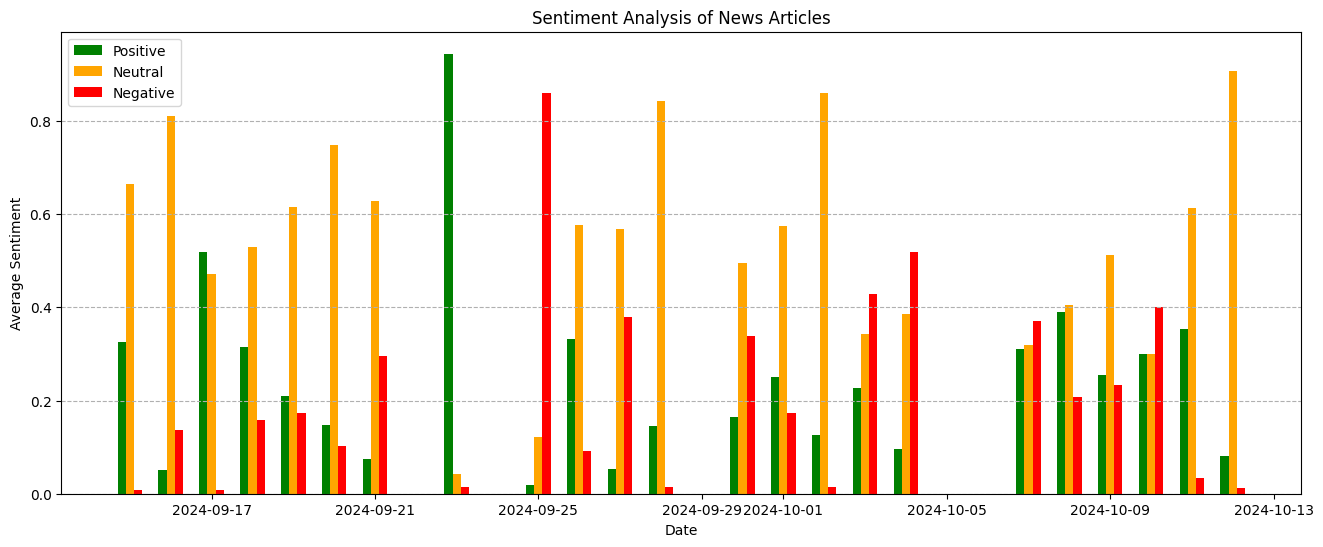
\includegraphics[width=0.85\linewidth]{gfx/m5l2_img001.png}
\par\smallskip{\small \textbf{Hình:} Cảm xúc trung bình của các bài báo theo ngày (tích cực, tiêu cực, trung lập).}
\end{figure}

Biểu đồ thu được là biểu đồ cột thể hiện cảm xúc trung bình của các bài báo theo thời gian. Mỗi ngày có ba cột, đại diện cho ba loại cảm xúc: tích cực (xanh lá), tiêu cực (đỏ) và trung lập (cam). Chiều cao của mỗi cột cho biết độ lớn của điểm cảm xúc trung bình thuộc loại đó vào ngày tương ứng. Cột càng cao thì cảm xúc càng mạnh.

Biểu đồ cho phép chúng ta quan sát xu hướng cảm xúc theo thời gian. Chúng ta có thể thấy cảm xúc trung bình thay đổi như thế nào qua các ngày, tức là đang trở nên tích cực hơn, tiêu cực hơn hay giữ ở mức trung lập. Bằng cách so sánh chiều cao các cột của từng loại, chúng ta có thể xác định những giai đoạn có cảm xúc tích cực hoặc tiêu cực mạnh hơn. Chẳng hạn, nếu vào một ngày nào đó cột đỏ (tiêu cực) cao hơn nhiều so với cột xanh lá (tích cực), điều này cho thấy các bài báo của ngày đó nhìn chung mang cảm xúc tiêu cực hơn. Ngược lại, cột xanh lá cao hơn sẽ cho thấy cảm xúc tích cực hơn.

\subsection{Điểm phân tích cảm xúc kết hợp với giá cổ phiếu}

Hãy xem xét ví dụ sau để thấy cách sử dụng điểm phân tích cảm xúc kết hợp với giá cổ phiếu của Microsoft, đồng thời lưu ý các hạn chế về độ chính xác của phân tích cảm xúc và nhu cầu sử dụng thêm các công cụ phân tích khác.

Trong ví dụ này, chúng ta sẽ trực quan hóa xu hướng của cảm xúc và giá. Chúng ta sẽ vẽ điểm cảm xúc cùng với giá cổ phiếu lịch sử. Điều này có thể giúp nhận diện bằng mắt thường những tương quan tiềm năng giữa các thay đổi về cảm xúc và biến động giá.

\begin{lstlisting}[language=Python,escapeinside={(*@}{@*)}]
# Fetch Microsoft stock data for the same date range
msft = yf.download("MSFT", start=df_grouped.index.min(), end=df_grouped.index.max())

# Scale the Microsoft price data
scaler = MinMaxScaler()
scaled_stock_price = scaler.fit_transform(msft[['Close']])

# Plot scaled price plot
fig, ax = plt.subplots(figsize=(16, 6))
ax.plot(msft.index, scaled_stock_price, color='blue', label='MSFT Adj Close Price (Scaled)')

# Plot the sentiment data
width = 0.2  # Adjust the width as needed
ax.bar(df_grouped.index - pd.DateOffset(days=width), df_grouped['avg_negative'], width=width, label='Negative', color='red')
ax.bar(df_grouped.index, df_grouped['avg_neutral'], width=width, label='Neutral', color='orange')
ax.bar(df_grouped.index + pd.DateOffset(days=width), df_grouped['avg_positive'], width=width, label='Positive', color='green')

# Set plot attributes (labels, ticks, title, legend, gridlines)
ax.set_xlabel('Date')
ax.set_title('Sentiment Analysis and Stock Price of Microsoft (scaled)')
ax.set_ylabel('Value (Sentiment and Stock Price)')
ax.legend()
ax.grid(True, axis='y', linestyle='--')
plt.show()
\end{lstlisting}

Giờ đây biểu đồ cũng hiển thị giá cổ phiếu của Microsoft cùng với các cột điểm cảm xúc. Lưu ý rằng giá cổ phiếu đã được chuẩn hóa tỷ lệ, và chúng ta thực hiện việc này bằng MinMaxScaler. MinMaxScaler từ \texttt{sklearn.preprocessing} đưa dữ liệu về một khoảng giá trị xác định, thường là từ 0 đến 1. Nó thực hiện điều này bằng cách áp dụng công thức sau:

\[X_{\text{scaled}} = \frac{(X - X_{min})}{(X_{max} - X_{min})}\]

Trong đó:

\begin{itemize}
\item
  \(X\) là dữ liệu gốc;
\item
  \(X_{\text{scaled}}\) là dữ liệu đã chuẩn hóa tỷ lệ;
\item
  \(X_{min}\) là giá trị nhỏ nhất của mỗi đặc trưng (cột) trong \(X\);
\item
  \(X_{max}\) là giá trị lớn nhất của mỗi đặc trưng (cột) trong \(X\);
\end{itemize}

Điều này có nghĩa là điểm dữ liệu có giá trị lớn nhất trong dữ liệu gốc sẽ được chuẩn hóa thành 1. Điểm dữ liệu có giá trị nhỏ nhất trong dữ liệu gốc sẽ được chuẩn hóa thành 0. Và tất cả các điểm dữ liệu còn lại sẽ được chuẩn hóa theo tỷ lệ giữa 0 và 1 dựa trên vị trí tương đối của chúng trong khoảng giá trị của dữ liệu gốc.

Mặc dù giá cổ phiếu đã chuẩn hóa không cho thấy các giá trị giá thực tế, nó vẫn biểu diễn biến động giá cổ phiếu theo cách đã được chuẩn hóa, cho phép chúng ta tập trung vào các xu hướng và mô hình, đồng thời so sánh chúng với các đặc trưng đã chuẩn hóa khác. Khi vẽ giá cổ phiếu đã chuẩn hóa cùng với điểm cảm xúc, về bản chất chúng ta đang so sánh các xu hướng và mô hình của cả hai đặc trưng theo thời gian. Chúng ta có thể quan sát xem cảm xúc tích cực có xu hướng trùng với các biến động giá tăng hay không, cảm xúc tiêu cực có trùng với các biến động giảm hay không, hoặc liệu có bất kỳ mối quan hệ thú vị nào khác.

\section{Kịch bản: Mô hình hóa chủ đề của tin tức tài chính}

Giờ đây, chúng ta sẽ sử dụng dữ liệu từ News API để khám phá các chủ đề tiềm ẩn trong các bài báo tài chính liên quan đến Microsoft và phân tích cảm xúc gắn với từng chủ đề.

\textbf{Mô hình hóa chủ đề} (topic modeling) là một kỹ thuật học máy không giám sát dùng để khám phá các cấu trúc chủ đề hay các chủ đề tiềm ẩn trong một tập hợp văn bản (còn gọi là \textbf{kho ngữ liệu}, corpus). Kỹ thuật này nhằm tự động nhận diện các nhóm từ thường xuyên xuất hiện cùng nhau trong các văn bản, đại diện cho những chủ đề hoặc nội dung nền tảng. Các thuật toán mô hình hóa chủ đề thường hoạt động dựa trên giả định rằng mỗi văn bản là sự pha trộn của một số ít chủ đề, và mỗi chủ đề được đặc trưng bởi một phân phối của các từ. Mục tiêu là học các phân phối chủ đề này cùng với việc gán chủ đề cho từng văn bản.

Các thuật ngữ chính:

\begin{itemize}
\item
  \textbf{Văn bản (Document):} Một đơn vị văn bản đơn lẻ, chẳng hạn như một bài báo, một bài đăng blog hoặc một tweet.
\item
  \textbf{Kho ngữ liệu (Corpus):} Một tập hợp các văn bản.
\item
  \textbf{Chủ đề (Topic):} Một cấu trúc chủ đề tiềm ẩn trong kho ngữ liệu, được biểu diễn bằng một phân phối của các từ.
\item
  \textbf{Phân phối văn bản-chủ đề (Document-Topic Distribution):} Xác suất hoặc trọng số của từng chủ đề trong mỗi văn bản.
\item
  \textbf{Phân phối chủ đề-từ (Topic-Word Distribution):} Xác suất hoặc trọng số của từng từ trong mỗi chủ đề.
\end{itemize}

Phân rã ma trận không âm (NMF) là một kỹ thuật mạnh mẽ để khám phá các chủ đề tiềm ẩn trong dữ liệu văn bản. Khi áp dụng vào tin tức tài chính, chúng ta có thể phát hiện các chủ đề chính đang được thảo luận về Microsoft. Việc kết hợp mô hình hóa chủ đề với phân tích cảm xúc giúp hiểu sâu hơn về cảm xúc gắn với các chủ đề khác nhau. Điều này có thể giúp xác định những lĩnh vực mà công ty nhận được nhận định tích cực hoặc tiêu cực. Những hiểu biết thu được từ phân tích này có thể hỗ trợ các quyết định đầu tư, quản trị rủi ro và chiến lược quan hệ công chúng.

\textbf{Các bước triển khai:}

\begin{itemize}
\item
  \textbf{Chuẩn bị dữ liệu:} Chúng ta sẽ sử dụng DataFrame \texttt{df} hiện có chứa dữ liệu News API, chọn cột \textquotesingle Description\textquotesingle{} làm dữ liệu văn bản để phân tích. Chúng ta sẽ tiền xử lý dữ liệu văn bản (loại bỏ từ dừng, dấu câu, rút gọn gốc từ/chuẩn hóa từ vựng).
\item
  \textbf{Tạo ma trận văn bản-thuật ngữ (TDM):} Sau đó, chúng ta sẽ tạo ma trận văn bản-thuật ngữ bằng TF-IDF (Term Frequency-Inverse Document Frequency). Ma trận này biểu diễn tần suất hoặc mức độ quan trọng của từng từ trong mỗi văn bản.
\item
  \textbf{Áp dụng NMF:} Chúng ta áp dụng NMF lên ma trận văn bản-thuật ngữ để phân rã thành hai ma trận: ma trận \(W\) biểu diễn mức độ quan trọng của từng chủ đề trong mỗi văn bản và ma trận \(H\) biểu diễn mức độ quan trọng của từng từ trong mỗi chủ đề.
\item
  \textbf{Trích xuất và diễn giải chủ đề:} Truy cập ma trận chủ đề-từ (\(H\)) để xem xét các từ hàng đầu của từng chủ đề. Xác định các từ có trọng số cao nhất trong mỗi hàng của \(H\) để hiểu nội dung của từng chủ đề. Dựa trên các từ hàng đầu, chúng ta đặt tên có ý nghĩa cho các chủ đề để dễ diễn giải.
\item
  \textbf{Gán chủ đề cho văn bản:} Lấy ma trận văn bản-chủ đề (\(W\)) để gán chủ đề chiếm ưu thế cho các văn bản. Với mỗi văn bản, chúng ta tìm chủ đề có trọng số cao nhất trong hàng tương ứng của \(W\). Cách này gán chủ đề nổi bật nhất cho mỗi văn bản.
\end{itemize}

\subsection{Chuẩn bị dữ liệu}

Chúng ta bắt đầu với bước chuẩn bị dữ liệu. Chúng ta tiền xử lý cột \textquotesingle Description\textquotesingle{} bằng hàm \texttt{preprocess()} đã giới thiệu ở trên và lưu mỗi mô tả đã xử lý vào một cột mới có tên \textquotesingle Processed\_Description\textquotesingle:

\begin{lstlisting}[language=Python,escapeinside={(*@}{@*)}]
# Preprocessing 'Description' column in df
df.loc[:, 'Processed_Description'] = df['Description'].apply(lambda x: preprocess(x))
\end{lstlisting}

Sau đó, chúng ta sẵn sàng áp dụng kỹ thuật Tần suất từ - Nghịch đảo tần suất văn bản (Term Frequency-Inverse Document Frequency, TF-IDF).

\subsection{Trích xuất đặc trưng - Ma trận tài liệu-thuật ngữ (TDM)}

Trong đoạn mã sau, chúng ta khớp (fit) bộ vector hóa \texttt{TfidfVectorizer} với dữ liệu trong cột \textquotesingle Processed\_Description\textquotesingle. Chúng ta áp dụng \texttt{TfidfVectorizer} với tham số \texttt{max\_features=250}, giới hạn kích thước từ vựng ở 250 từ xuất hiện thường xuyên nhất. Điều này giúp giảm số chiều của ma trận tài liệu-thuật ngữ (DTM) và có thể cải thiện hiệu năng. Chúng ta cũng dùng tham số \texttt{stop\_words=\textquotesingle{}english\textquotesingle{}} để loại bỏ các từ tiếng Anh thông dụng (như "the," "a," "is") khỏi từ vựng, vì chúng thường không mang nhiều thông tin có ý nghĩa. Thao tác này sẽ chuyển dữ liệu văn bản trong \textquotesingle Processed\_Description\textquotesingle{} thành ma trận tài liệu-thuật ngữ (DTM), được biểu diễn bằng biến \texttt{dtm}:

\begin{lstlisting}[language=Python,escapeinside={(*@}{@*)}]
# TF-IDF Vectorization
vectorizer = TfidfVectorizer(max_features=250, stop_words='english')
dtm = vectorizer.fit_transform(df['Processed_Description'])
dtm.shape
\end{lstlisting}

Biến \texttt{dtm} lúc này chứa một ma trận thưa, trong đó:

\begin{itemize}
\item
  Mỗi hàng đại diện cho một tài liệu (trong trường hợp của chúng ta là một bài báo tin tức).
\item
  Mỗi cột đại diện cho một từ (hay đặc trưng) trong từ vựng.
\item
  Các giá trị trong ma trận biểu thị điểm TF-IDF của từng từ trong từng tài liệu.
\item
  \texttt{dtm} thường được lưu dưới dạng ma trận thưa để tiết kiệm bộ nhớ vì nó thường chứa nhiều giá trị bằng không.
\end{itemize}

Phạm vi thông thường của \texttt{max\_features} là từ 1000 đến 5000, nhưng có thể thay đổi rất nhiều tùy theo tập dữ liệu và tác vụ, dựa trên các yếu tố như kích thước tập dữ liệu, độ phức tạp của tác vụ, tài nguyên tính toán, thực nghiệm, v.v. Với một tập dữ liệu như của chúng ta chỉ có khoảng 90 hàng, giá trị \texttt{max\_features} từ 100 đến 500 có lẽ là điểm khởi đầu phù hợp để cân bằng giữa số chiều và lượng thông tin.

\subsection{Áp dụng NMF}

Sau khi tạo \texttt{dtm}, giờ đây chúng ta có thể áp dụng NMF lên ma trận này để khám phá các chủ đề tiềm ẩn trong các bài báo tin tức tài chính. Chúng ta sẽ thực hiện việc này với tham số \texttt{n\_components=5}, tham số quy định số lượng chủ đề (hay thành phần) mà ta muốn trích xuất từ dữ liệu. Trong trường hợp này, ta nhắm đến năm chủ đề. \texttt{random\_state=42} đặt một hạt giống ngẫu nhiên (random seed) để đảm bảo khả năng tái lập kết quả. Việc dùng cùng một hạt giống bảo đảm ta thu được cùng một kết quả mỗi lần chạy mã:

\begin{lstlisting}[language=Python,escapeinside={(*@}{@*)}]
# NMF
nmf_model = NMF(n_components=5, random_state=42) # 5 topics
W = nmf_model.fit_transform(dtm)
H = nmf_model.components_
\end{lstlisting}

NMF được dùng để khám phá các chủ đề tiềm ẩn trong dữ liệu văn bản. Phương pháp này phân rã ma trận tài liệu-thuật ngữ thành hai ma trận có số chiều thấp hơn, biểu diễn mối quan hệ giữa từ và chủ đề, cũng như giữa chủ đề và tài liệu. Giờ đây chúng ta đã thu được:

\begin{itemize}
\item
  \(W\) (Ma trận Tài liệu-Chủ đề) biểu diễn phân phối của các chủ đề trong từng tài liệu. Mỗi hàng của \(W\) tương ứng với một tài liệu trong kho ngữ liệu, và mỗi cột tương ứng với một chủ đề do NMF khám phá. Các giá trị trong \(W\) cho biết trọng số hay xác suất xuất hiện của từng chủ đề trong mỗi tài liệu.
\item
  \(H\) (Ma trận Chủ đề-Từ) biểu diễn phân phối của các từ trong từng chủ đề. Mỗi hàng của \(H\) tương ứng với một chủ đề, và mỗi cột tương ứng với một từ trong từ vựng. Các giá trị trong \(H\) cho biết trọng số hay mức độ quan trọng của từng từ trong mỗi chủ đề.
\end{itemize}

Tham số \texttt{n\_components=5} xác định số lượng chủ đề (hay thành phần) mà ta muốn trích xuất từ dữ liệu. Trong trường hợp của chúng ta, ta nhắm đến việc khám phá năm chủ đề riêng biệt trong các bài báo tin tức tài chính liên quan đến Microsoft. Số lượng chủ đề nhỏ (như năm) thường cho kết quả dễ diễn giải hơn. Việc hiểu và gán nhãn có ý nghĩa cho năm chủ đề dễ dàng hơn so với, chẳng hạn, 20 hay 50 chủ đề. Khi mới bắt đầu với mô hình hóa chủ đề, thông thường nên bắt đầu với số lượng chủ đề nhỏ rồi tăng dần nếu cần. Cách này giúp nắm được bức tranh tổng quát về các chủ đề chính trong dữ liệu trước khi đi vào phân tích chi tiết hơn. Số lượng chủ đề nhỏ cũng làm giảm chi phí tính toán của NMF, giúp quá trình nhanh hơn, đặc biệt với các tập dữ liệu lớn hơn.

\subsection{Trích xuất và diễn giải chủ đề}

Bây giờ, chúng ta hãy xem xét các từ hàng đầu trong mỗi chủ đề để hiểu nội dung của chủ đề đó. Mục tiêu là hiểu các nội dung hay đối tượng mà năm chủ đề do NMF trích xuất đại diện.

Hãy nhớ rằng ma trận \(H\) lưu trữ trọng số của mỗi từ trong mỗi chủ đề. Chúng ta muốn xác định các từ có trọng số cao nhất cho từng chủ đề, vì những từ này đại diện tốt nhất cho nội dung của chủ đề. Với mỗi chủ đề, chúng ta sẽ hiển thị \(n\) từ hàng đầu có trọng số cao nhất. Điều này cho ta một cái nhìn sơ lược về đề tài của chủ đề. Dựa trên các từ hàng đầu, chúng ta sẽ cố gắng gán một nhãn hoặc cách diễn giải có ý nghĩa cho từng chủ đề. Việc này đòi hỏi kiến thức chuyên ngành và sự cân nhắc kỹ lưỡng về bối cảnh của các bài báo tin tức tài chính.

\begin{lstlisting}[language=Python,escapeinside={(*@}{@*)}]
# Retrieves the names of the features (words)
feature_names = vectorizer.get_feature_names_out()

# Extract top words
n_top_words = 10  # Top 10 words
for topic_idx, topic in enumerate(H):
    print(f"\nTopic {topic_idx + 1}:")
    print(" ".join([feature_names[i]
                    for i in topic.argsort()[:-n_top_words - 1:-1]]))
\end{lstlisting}

Chúng ta cũng có thể vẽ biểu đồ các từ hàng đầu của từng chủ đề để trực quan hóa tốt hơn. Trong đoạn mã sau, chúng ta vẽ 10 từ hàng đầu của mỗi chủ đề dưới dạng các biểu đồ cột con:

\begin{lstlisting}[language=Python,escapeinside={(*@}{@*)}]
# Set figure size
fig, axes = plt.subplots(1, nmf_model.n_components, figsize=(16, 6), sharex=True)
axes = axes.flatten()  # Convert to 1D array for easier indexing

# Plot bar subplots for each topic
for topic_idx, topic in enumerate(H):
    top_features_ind = topic.argsort()[:-n_top_words - 1:-1]
    top_features = [feature_names[i] for i in top_features_ind]
    weights = topic[top_features_ind]

    ax = axes[topic_idx]
    ax.barh(top_features, weights, height=0.5, fill='blue')
    ax.set_title(f'Topic {topic_idx + 1}', fontdict={'fontsize': 14})
    ax.invert_yaxis()
    ax.tick_params(axis='both', which='major', labelsize=12)

# Set figure attributes (title)
fig.suptitle('Top words in topics in NMF model', fontsize=20, y=0.98)
fig.tight_layout(h_pad=2.0)
plt.show()
\end{lstlisting}

Mục đích chính của đoạn mã này là hiển thị các từ hàng đầu của từng chủ đề do NMF trích xuất. Điều này giúp diễn giải các chủ đề và hiểu những nội dung hay đối tượng mà chúng đại diện.

Tại thời điểm viết bài, chúng tôi thu được các từ hàng đầu sau cho từng chủ đề (bạn có thể nhận được kết quả khác vì News API sẽ có một tập bài báo khác vào lúc bạn chạy đoạn mã này):

\begin{itemize}
\item
  \textbf{Chủ đề 1: Microsoft Windows và các tính năng AI}

  \begin{itemize}
    \item
    Từ hàng đầu: \texttt{copilot,\ plus,\ feature,\ new,\ pcs,\ features,\ search,\ voice,\ ai,\ windows}
  \item
    Diễn giải: Chủ đề này dường như liên quan đến các tính năng và cải tiến mới trong Microsoft Windows, đặc biệt là những tính năng liên quan đến AI và khả năng tìm kiếm bằng giọng nói. Copilot, một trợ lý AI mới có thể xuất hiện, cũng là một nội dung nổi bật.
  \end{itemize}
\item
  \textbf{Chủ đề 2: Các trung tâm dữ liệu và sáng kiến năng lượng của Microsoft}

  \begin{itemize}
    \item
    Từ hàng đầu: \texttt{data,\ energy,\ centers,\ power,\ nuclear,\ ai,\ tech,\ run,\ microsoft,\ carbon}
  \item
    Diễn giải: Chủ đề này dường như tập trung vào các trung tâm dữ liệu của Microsoft và mức tiêu thụ năng lượng của chúng. Chủ đề có thể bao gồm các thảo luận về nguồn điện, trong đó có năng lượng hạt nhân, và các sáng kiến nhằm giảm phát thải carbon. Việc sử dụng công nghệ AI trong các trung tâm dữ liệu cũng có thể là một nội dung đáng chú ý.
  \end{itemize}
\item
  \textbf{Chủ đề 3: Các nỗ lực AR/VR của Microsoft (Hololens)}

  \begin{itemize}
    \item
    Từ hàng đầu: \texttt{microsoft,\ windows,\ hololens,\ headsets,\ according,\ vr,\ update,\ production,\ uploadvr,\ 11}
  \item
    Diễn giải: Chủ đề này có khả năng xoay quanh các nỗ lực về thực tế tăng cường và thực tế ảo của Microsoft, đặc biệt tập trung vào kính Hololens. Chủ đề có thể bao gồm các cập nhật về sản xuất Hololens, các tính năng mới, hoặc quan hệ hợp tác với các nền tảng liên quan đến VR như UploadVR.
  \end{itemize}
\item
  \textbf{Chủ đề 4: Cạnh tranh trong lĩnh vực AI (Microsoft, OpenAI, Google)}

  \begin{itemize}
    \item
    Từ hàng đầu: \texttt{openai,\ google,\ ai,\ microsoft,\ stay,\ date,\ financial,\ way,\ competition,\ amid}
  \item
    Diễn giải: Chủ đề này xoay quanh sự cạnh tranh trong lĩnh vực trí tuệ nhân tạo, chủ yếu liên quan đến Microsoft, OpenAI và Google. Chủ đề có thể thảo luận về các khía cạnh tài chính, quan hệ đối tác chiến lược và bức tranh tổng thể của cuộc đua AI.
  \end{itemize}
\item
  \textbf{Chủ đề 5: Microsoft Flight Simulator và trò chơi điện tử}

  \begin{itemize}
    \item
    Từ hàng đầu: \texttt{flight,\ game,\ simulator,\ microsoft,\ 2024,\ test,\ based,\ reboot,\ 2020,\ office}
  \item
    Diễn giải: Chủ đề này dường như liên quan đến Microsoft Flight Simulator, một trò chơi mô phỏng bay phổ biến. Chủ đề có thể bao gồm các thảo luận về bản cập nhật, tính năng mới, các giai đoạn thử nghiệm hoặc những bản phát hành tiềm năng trong tương lai. Việc xuất hiện từ "office" hơi bất thường và có thể cần thêm ngữ cảnh để hiểu mức độ liên quan của nó.
  \end{itemize}
\end{itemize}

Dựa trên các diễn giải này, dưới đây là một bộ nhãn được đề xuất cho các chủ đề:

\begin{enumerate}
\def\labelenumi{\arabic{enumi}.}
\item
  Cải tiến AI trong Windows
\item
  Tính bền vững của trung tâm dữ liệu
\item
  Hololens và AR/VR
\item
  Cạnh tranh trong ngành AI
\item
  Flight Simulator và trò chơi điện tử
\end{enumerate}

Các nhãn này thể hiện ngắn gọn và đầy đủ thông tin các nội dung mà từng chủ đề nắm bắt được. Hãy nhớ rằng việc diễn giải chủ đề có thể mang tính chủ quan, vì vậy các nhãn có thể được điều chỉnh dựa trên cách hiểu của riêng bạn về dữ liệu và bối cảnh.

Bằng cách phân tích cẩn thận các từ hàng đầu và xem xét bối cảnh rộng hơn, chúng ta có thể thu được những hiểu biết giá trị về các nội dung chính được thảo luận trong các bài báo tin tức tài chính liên quan đến Microsoft.

\subsection{Gán chủ đề cho tài liệu}

Bây giờ, chúng ta sẽ dùng \texttt{W} để gán chủ đề nổi bật nhất cho từng tài liệu. Ta có thể thực hiện bằng cách tìm chủ đề (cột) có trọng số cao nhất đối với mỗi tài liệu (hàng) trong \texttt{W}:

\begin{lstlisting}[language=Python,escapeinside={(*@}{@*)}]
# Assigns the dominant topic for each document
df['Dominant_Topic'] = W.argmax(axis=1) + 1  # +1 to start topic numbering from 1
\end{lstlisting}

Ở đây, \texttt{W.argmax(axis=1)} tìm chỉ số của giá trị lớn nhất (trọng số cao nhất) trong mỗi hàng của \(W\). Chỉ số này tương ứng với chủ đề chiếm ưu thế của tài liệu đó. Còn \texttt{+\ 1} cộng thêm 1 vào chỉ số chủ đề để việc đánh số chủ đề bắt đầu từ 1 thay vì 0 (mặc định trong cách đánh chỉ số của Python).

Biểu đồ cột có thể được dùng để trực quan hóa phân phối các chủ đề trong từng tài liệu riêng lẻ hoặc trên toàn bộ kho ngữ liệu. Biểu đồ cột sau đây thể hiện phân phối chủ đề trung bình trên tất cả các tài liệu:

\begin{lstlisting}[language=Python,escapeinside={(*@}{@*)}]
# Visualize average topic distribution across all documents
avg_topic_distribution = W.mean(axis=0)

# Define topic labels
topic_labels = ["Windows AI Enhancements", "Data Center Sustainability",
                "Hololens and AR/VR", "AI Industry Competition",
                "Flight Simulator and Gaming"]

# Create bar plot
bars = plt.bar(np.arange(nmf_model.n_components) + 1, avg_topic_distribution, color='skyblue')

# Add bar labels inside bars
for bar, label in zip(bars, topic_labels):
    plt.text(bar.get_x() + bar.get_width() / 2, bar.get_height() / 2, label,
             ha='center', va='center', rotation=90, color='black', fontsize=8)

plt.xticks(np.arange(nmf_model.n_components) + 1)
plt.xlabel("Topic")
plt.ylabel("Average Weight")
plt.title("Average Topic Distribution Across All Documents")
plt.show()
\end{lstlisting}

Biểu đồ cột này minh họa mức độ phổ biến trung bình của từng chủ đề trên tất cả các tài liệu trong tập dữ liệu. Chiều cao của mỗi cột biểu thị trọng số trung bình, hay mức độ quan trọng, của chủ đề đó trên toàn bộ các tài liệu được phân tích. Cột càng cao cho thấy chủ đề đó càng nổi bật hoặc được đề cập thường xuyên hơn xét trên tổng thể.

Dựa vào chiều cao của các cột tương ứng, ta có thể thấy "AI Industry Competition" là chủ đề phổ biến nhất, tiếp theo là "Hololens and AR/VR".

Thông qua việc xem xét trực quan hóa này, chúng ta có thể hiểu rõ hơn về phân bố chủ đề tổng thể trong tập dữ liệu. Thông tin này sẽ định hướng cho các phân tích tiếp theo, chẳng hạn tập trung vào các tài liệu liên quan đến "AI Industry Competition" và "Hololens and AR/VR" để hiểu sâu hơn về những chủ đề chủ đạo này.

\section{Kết luận}

Trong bài học này, chúng ta đã khảo sát các nguồn dữ liệu tin tức khác nhau. Chúng ta đã so sánh và đối chiếu các nguồn như yfinance, Google News RSS và News API. Cuối cùng, News API được lựa chọn nhờ tính linh hoạt và các tính năng của nó.

Sau đó, chúng ta thực hiện phân tích cảm xúc bằng FinBERT, một mô hình NLP được huấn luyện trước dành cho văn bản tài chính. Điểm số cảm xúc (tích cực, tiêu cực và trung lập) được tính cho các bài báo về Microsoft. Các điểm số cảm xúc được vẽ theo thời gian để quan sát xu hướng và các mối tương quan tiềm năng với giá cổ phiếu của Microsoft.

Cuối cùng, chúng ta áp dụng mô hình hóa chủ đề, sử dụng phân rã ma trận không âm (NMF) để khám phá các chủ đề hoặc nội dung chính tiềm ẩn trong dữ liệu tin tức. Quá trình này bao gồm tiền xử lý văn bản, tạo ma trận tài liệu-thuật ngữ bằng TF-IDF và áp dụng thuật toán NMF.

\begin{center}\rule{0.5\linewidth}{0.5pt}\end{center}

Bản quyền 2024 WorldQuant University. Nội dung này chỉ được cấp phép cho mục đích sử dụng cá nhân. Nghiêm cấm phân phối lại hoặc công bố tài liệu này.

\begin{lstlisting}[language=Python,escapeinside={(*@}{@*)}]

\end{lstlisting}
